\chapter{Grassmann path integrals and Feynman diagrams for Fermions}
\begin{itemize}
	\item Grassmann number 和 Gaussian-Berezin integrals 见 section \ref{B.2}.
\end{itemize}

\section{Grassmann path integral}
\begin{itemize}
	\item Dirac field 的 partition function 为
	\begin{align}
		Z(\eta, \bar{\eta}) &= \int D\Psi D\bar{\Psi} \, e^{i \int d^4 x \, (\bar{\Psi} (i \cancel{\partial} - m + i \epsilon) \Psi + \bar{\eta} \Psi + \bar{\Psi} \eta)} \notag \\
		&= e^{i E_0 T} e^{- i \int \frac{d^4 p}{(2 \pi)^4} \tilde{\bar{\eta}}(- p) \frac{1}{\cancel{p} - m + i \epsilon} \tilde{\eta}(p)},
	\end{align}
	其中 vacuum energy 为
	\begin{equation}
		E_0 = - 4 V \int \frac{d^3 p}{(2 \pi)^3} \frac{1}{2} \omega_p + \text{irrelevant terms}.
	\end{equation}
	
	\begin{tcolorbox}[title=calculation:]
		代入 \eqref{10.1.13},
		\begin{equation}
			Z(\eta, \bar{\eta}) = \det(\underbrace{i (i \cancel{\partial} - m + i \epsilon)}_{= i A}) e^{- i^2 (- i) \bar{\eta} A^{- 1} \eta},
		\end{equation}
		其中
		\begin{align}
			& \begin{dcases}
				\det(i (i \cancel{\partial} - m + i \epsilon)) = \det(i \underbrace{\gamma^5 (i \cancel{\partial} - m + i \epsilon) \gamma^5}_{= (- i \cancel{\partial} - m + i \epsilon)}) \\
				(i \cancel{\partial} - m + i \epsilon) (- i \cancel{\partial} - m + i \epsilon) = (\partial^2 + m^2 - i \epsilon) I_{4 \times 4}
			\end{dcases} \notag \\
			\Longrightarrow & \det(i (i \cancel{\partial} - m + i \epsilon)) = \sqrt{\det((- \partial^2 - m^2 + i \epsilon) I_{4 \times 4})} = e^{i E_0 T},
		\end{align}
		注意到 $I_{4 \times 4}$ 会带来一个 $4$ 次方的系数.
		
		\noindent\rule[0.5ex]{\linewidth}{0.5pt} % horizontal line
		
		对于指数项, 考虑
		\begin{equation}
			(i \cancel{\partial} - m + i \epsilon) \Psi(x) = \int d^4 y \, A(x - y) \Psi(y),
		\end{equation}
		其中
		\begin{align}
			& A(x - y) = \int \frac{d^4 p}{(2 \pi)^4} (\cancel{p} - m + i \epsilon) e^{- i p \cdot (x - y)} \notag \\
			\Longrightarrow & A^{- 1}(x - y) = S(x - y),
		\end{align}
		其中 $S(x - y)$ 是传播子, 见 \eqref{8.6.1}, 所以指数项为
		\begin{equation}
			e^{- i \bar{\eta} A^{- 1} \eta} = e^{- i \int d^4 x d^4 y \, \bar{\eta}(x) S(x - y) \eta(y)} = \cdots
		\end{equation}
	\end{tcolorbox}
\end{itemize}

\section{Feynman rules for Yukawa interaction}
\begin{itemize}
	\item 考虑如下 Lagrangian,
	\begin{equation}
		\mathcal{L} = \bar{\Psi} (i \cancel{\partial} - m) \Psi + \frac{1}{2} ((\partial \phi)^2 - \mu^2 \phi^2) - \frac{\lambda}{4!} \phi^4 + g \bar{\Psi} \phi \Psi,
	\end{equation}
	对应如下 partition function,
	\begin{align}
		\frac{Z(\bar{\eta}, \eta, J; \lambda, g)}{Z(0; 0)} =& e^{i \int d^4 x \, (- \frac{\lambda}{4!} (\frac{\delta}{\delta i J(x)})^4 + g \frac{\delta}{\delta i \eta_\alpha(x)} \frac{\delta}{\delta i J(x)} \frac{\delta}{\delta i \bar{\eta}_\alpha(x)})} e^{- \frac{i}{2} J D J - i \bar{\eta}_\alpha S_{\alpha \beta} \eta_\beta}, \quad \text{Schwinger's way}, \notag \\
		=& \sum_{l, m, n = 0}^\infty \frac{i^{l + m + n}}{l! m! n!} (- 1)^{\frac{m (m - 1) + n (n - 1)}{2}} \int d^4 x_1 \cdots d^4 x_l d^4 y_1 \cdots d^4 y_m d^4 z_1 \cdots d^4 z_n \notag \\
		& J(x_1) \cdots \bar{\eta}_{\alpha_1}(y_1) \cdots G^{(l, m, n)}_{\alpha_1 \cdots \beta_1 \cdots}(x_1, \cdots, z_n) \eta_{\beta_1}(z_1) \cdots, \quad \text{Weyl's way},
	\end{align}
	其中
	\begin{equation}
		G^{(l, m, n)}_{\alpha_1 \cdots \beta_1 \cdots}(x_1, \cdots, z_n) = e^{i \int d^4 x \, \mathcal{L}(\lambda, g)} \phi(x_1) \cdots \Psi_{\alpha_1}(y_1) \cdots \bar{\Psi}_{\beta_1}(z_1) \cdots
	\end{equation}
	
	\noindent\rule[0.5ex]{\linewidth}{0.5pt} % horizontal line
	
	\item 下面给出一些 Feynman diagrams 作为例子, 先用正则量子化方法计算, 首先,
	\begin{align}
		\vcenter{\hbox{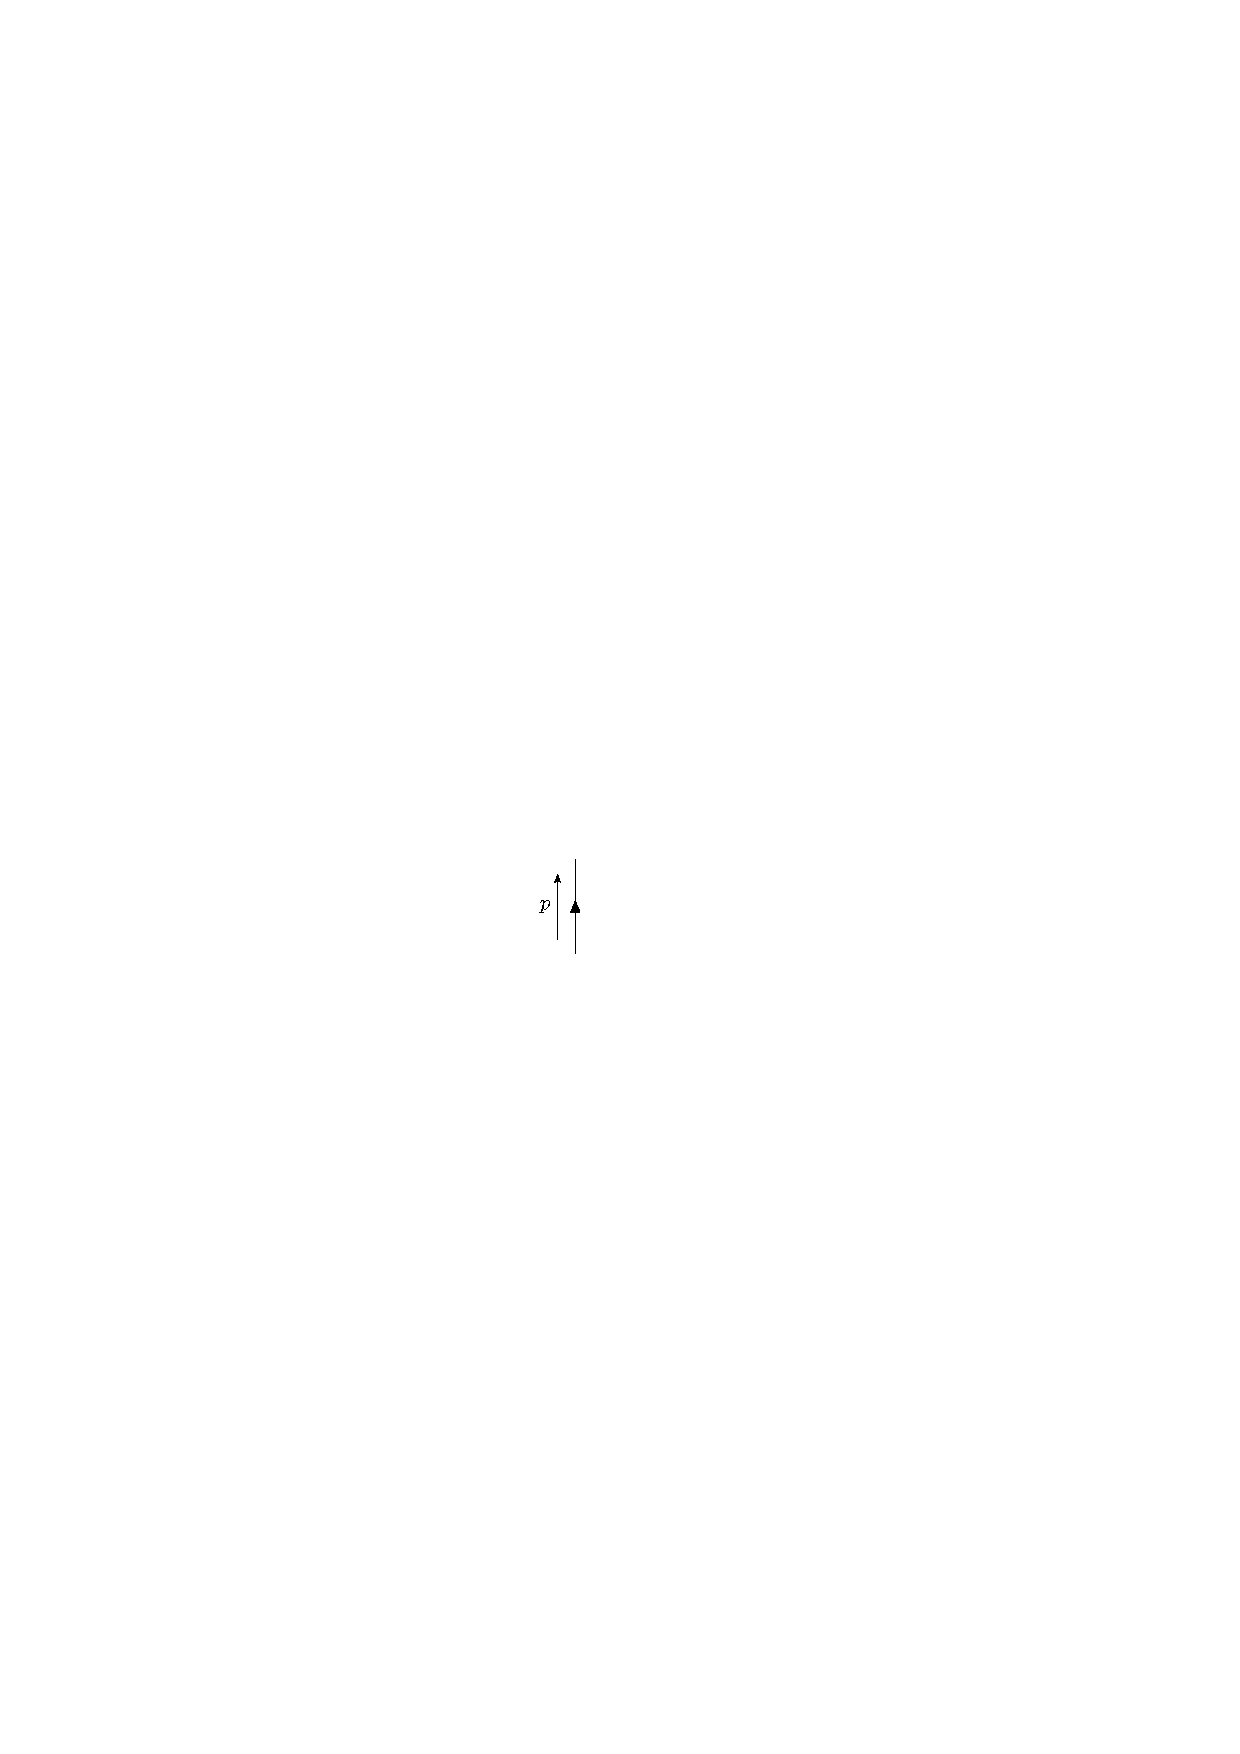
\includegraphics[scale=1]{figures/Yukawa interaction - Feynman diagram 1.pdf}}} &= \rho^2(p_1) \delta^{(3)}(\vec{p}_1 - \vec{p}_2) \delta_{s_1 s_2}, \\
		\vcenter{\hbox{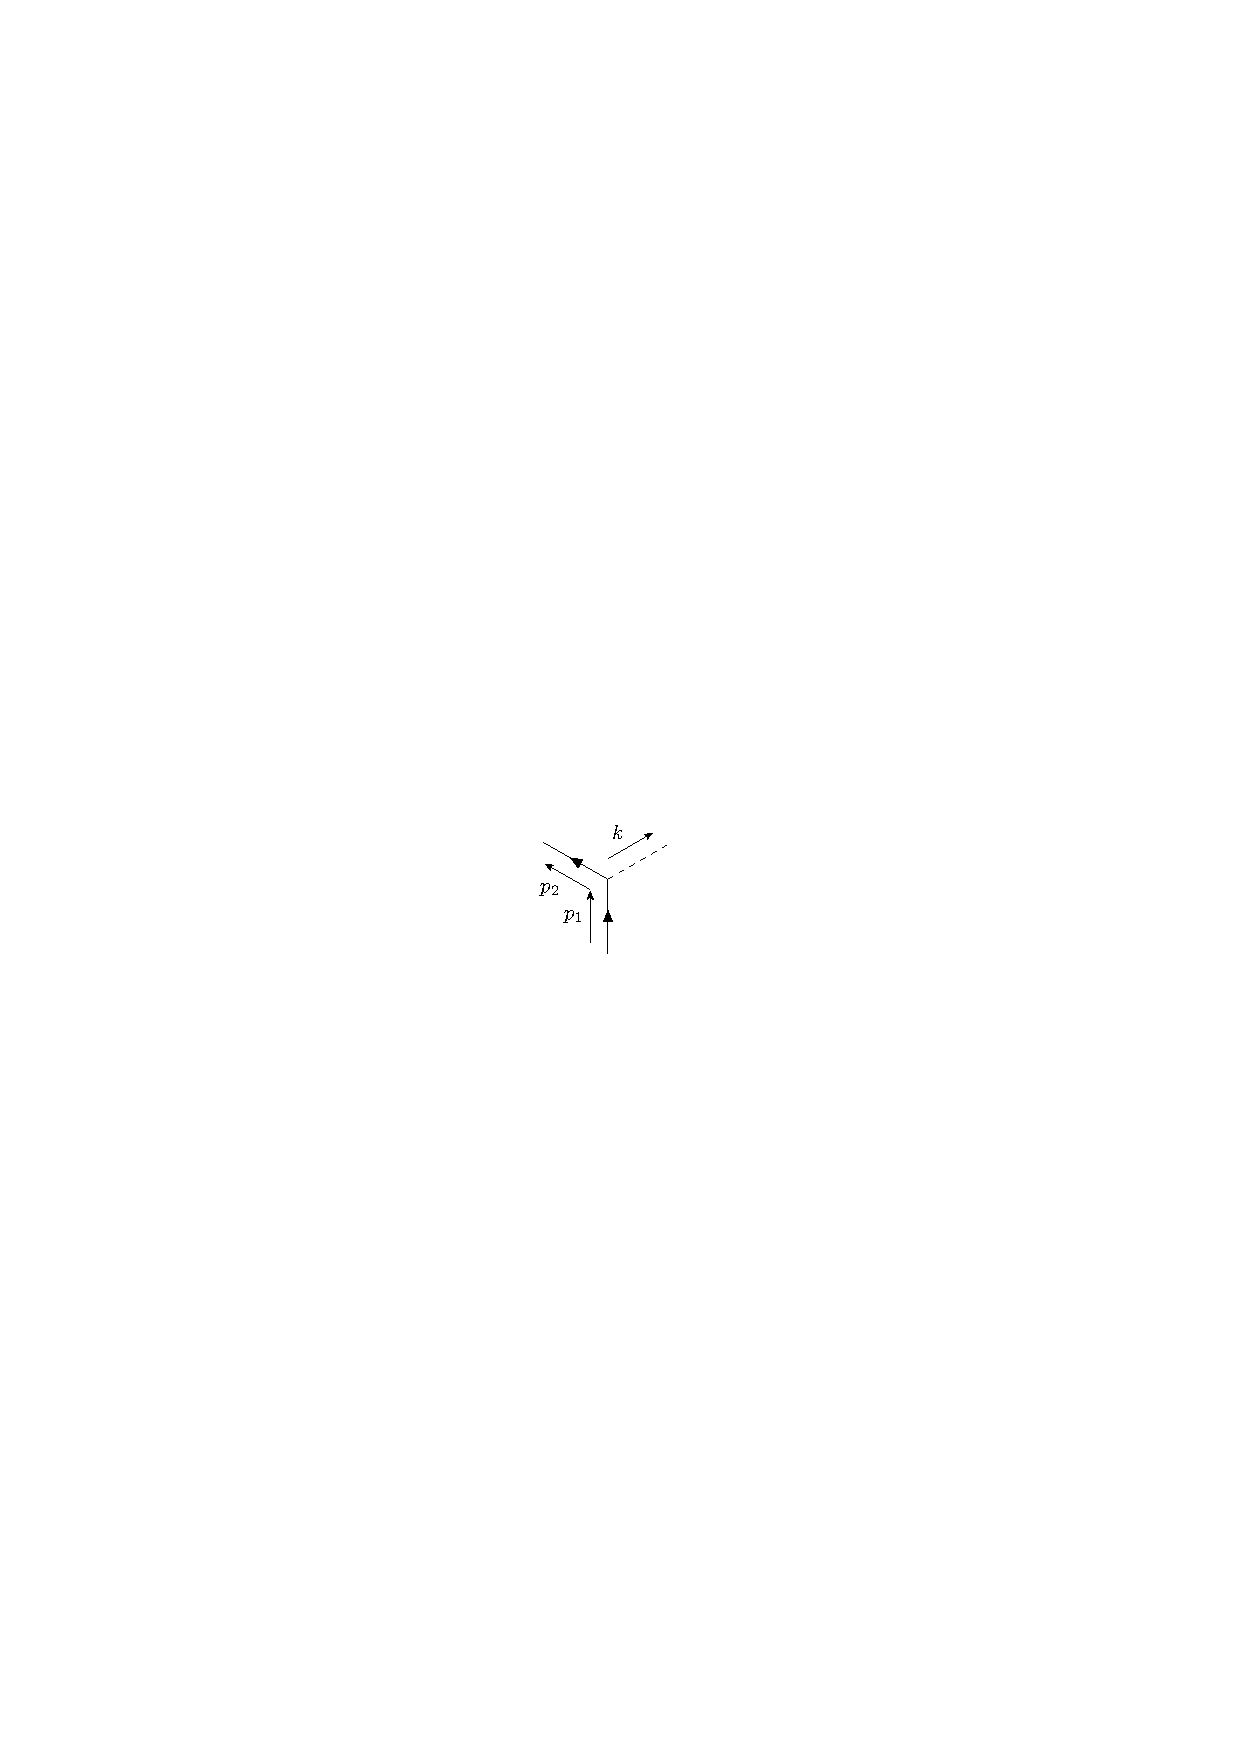
\includegraphics[scale=1]{figures/Yukawa interaction - Feynman diagram 2.pdf}}} &= \rho(p_1) \rho(p_2) \rho(k) (- i g) \int d^4 x \, \braket{0 | \wick{
			\c2 b^{s_2}_{\vec{p}_2} \c3 a_{\vec{k}} (\c2 {\bar{\Psi}}(x) \c3 \phi(x) \c1 \Psi(x)) \c1 b^{s_1 \dag}_{\vec{p}_1}
		} | 0} \notag \\
		&= (- i g) \int d^4 x \, e^{- i (p_1 - p_2 - k) \cdot x} \bar{u}(\vec{p}_2, s_2) u(\vec{p}_1, s_1),
	\end{align}
	再算一个复杂一点的例子,
	\begin{align}
		\vcenter{\hbox{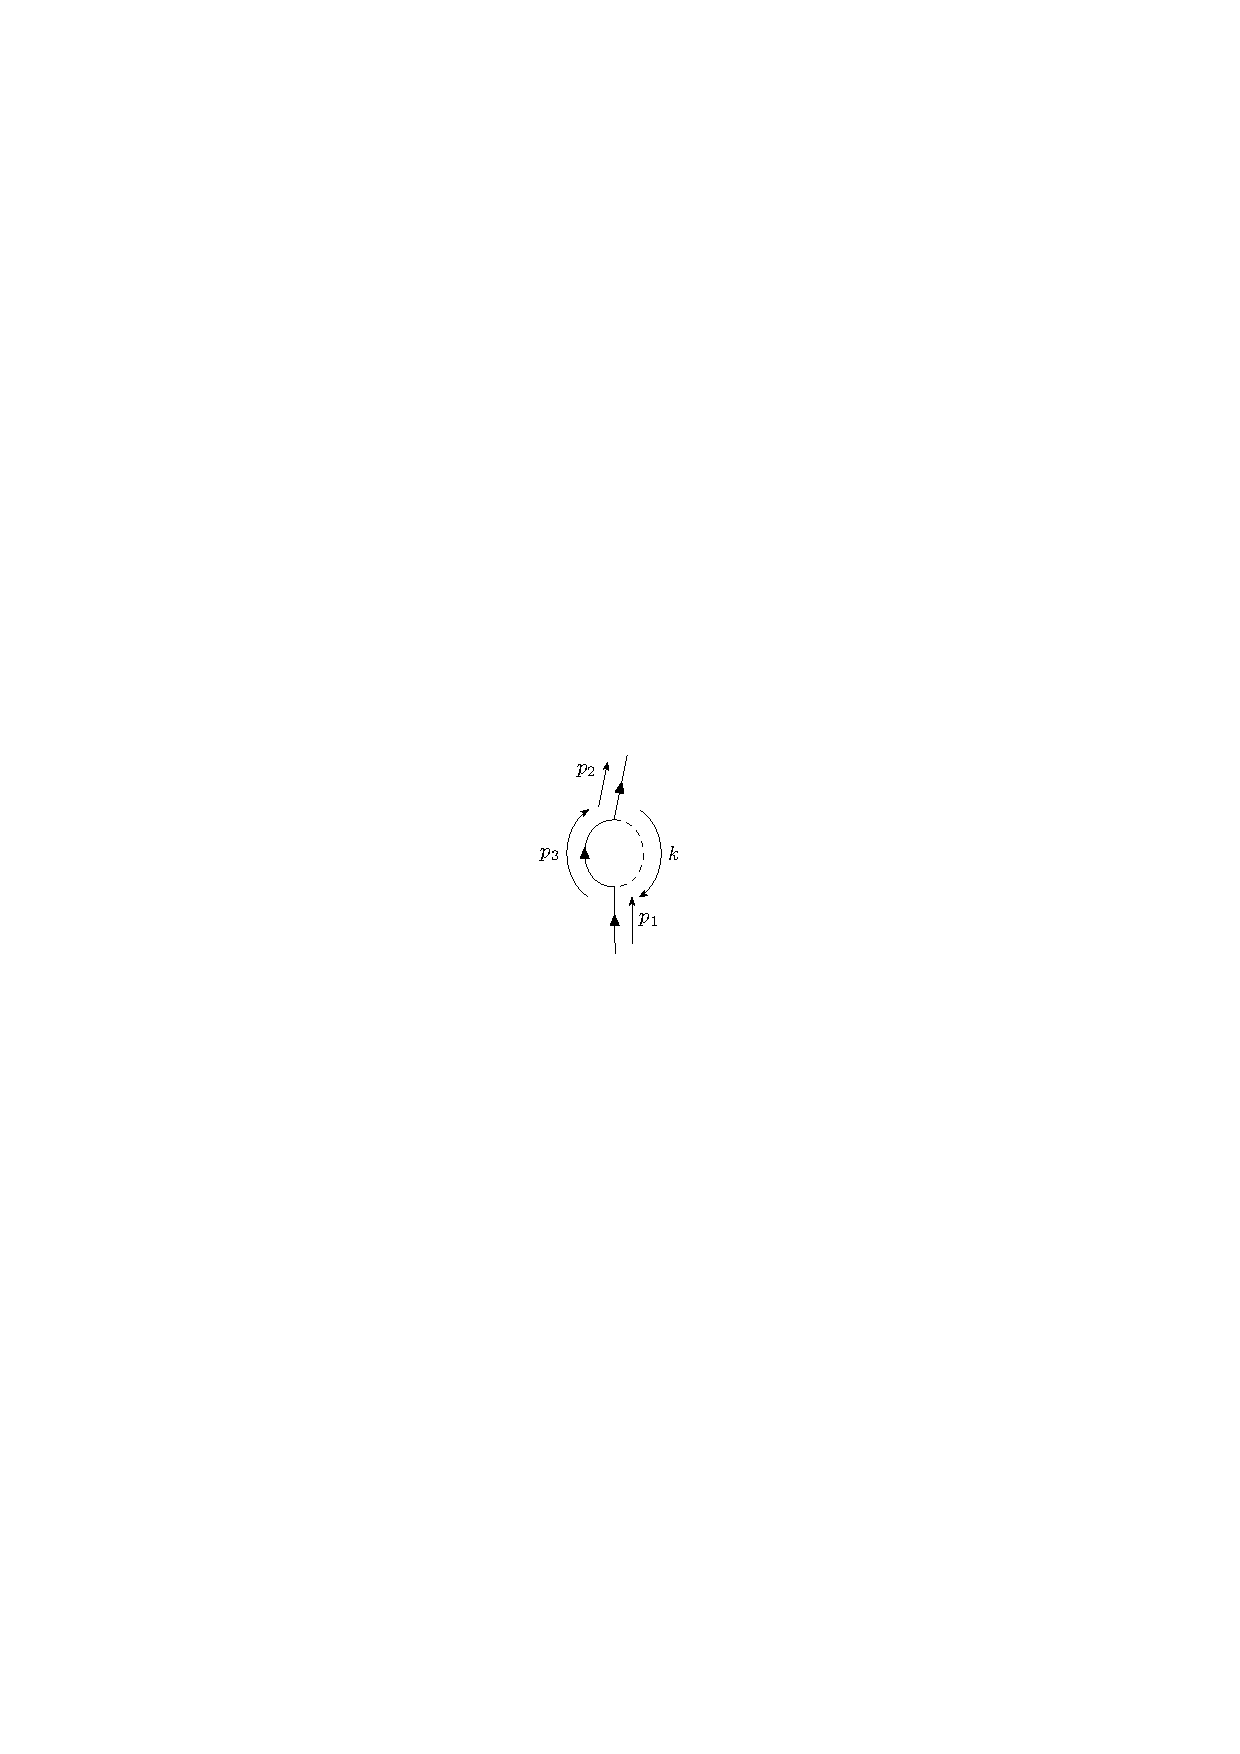
\includegraphics[scale=1]{figures/Yukawa interaction - Feynman diagram 3.pdf}}} =& (- i g)^2 (2 \pi)^4 \delta^{(4)}(p_1 - p_2) \notag \\
		& \bar{u}_\alpha(\vec{p}_2, s_2) \Big( \int \frac{d^4 p_3}{(2 \pi)^4} \frac{i}{\cancel{p}_3 - m + i \epsilon} \frac{i}{(p_2 - p_3)^2 - \mu^2 + i \epsilon} \Big)_{\alpha \beta} u_\beta(\vec{p}_1, s_1). \label{10.2.5}
	\end{align}
	
	\begin{tcolorbox}[title=calculation:]
		注意不要忘了算符按时间排序,
		\begin{align}
			& \cdots \notag \\
			=& \rho(p_1) \rho(p_2) \frac{(- i g)^2}{2!} \int d^4 x_1 d^4 x_2 \, \Big( \theta(t_1 - t_2) \Big( \braket{0 | \wick{
				\c2 b^{s_2}_{\vec{p}_2} (\c2 {\bar{\Psi}}(x_1) \c4 \phi(x_1) \c3 \Psi(x_1) \c3 {\bar{\Psi}}(x_2) \c4 \phi(x_2) \c1 \Psi(x_2)) \c1 b^{s_1 \dag}_{\vec{p}_1}
			} | 0} \notag \\
			& + \braket{0 | \wick{
				\c2 b^{s_2}_{\vec{p}_2} (\c3 {\bar{\Psi}}(x_1) \c4 \phi(x_1) \c1 \Psi(x_1) \c2 {\bar{\Psi}}(x_2) \c4 \phi(x_2) \c3 \Psi(x_2)) \c1 b^{s_1 \dag}_{\vec{p}_1}
			} | 0} \Big) - \theta(t_2 - t_1) \cdots \Big) \notag \\
			=& 2 \times \frac{(- i g)^2}{2!} \int d^4 x_1 d^4 x_2 \notag \\
			& e^{i (p_2 \cdot x_1 - p_1 \cdot x_2)} \bar{u}_\alpha(\vec{p}_2, s_2) \Big( \int \frac{d^4 p_3}{(2 \pi)^4} \frac{i e^{- i p_3 \cdot (x_1 - x_2)}}{\cancel{p}_3 - m + i \epsilon} \Big)_{\alpha \beta} u_\beta(\vec{p}_1, s_1) \int \frac{d^4 k}{(2 \pi)^4} \frac{i e^{- i k \cdot (x_1 - x_2)}}{k^2 - \mu^2 + i \epsilon} \notag \\
			=& (- i g)^2 (2 \pi)^4 \delta^{(4)}(p_1 - p_2) \notag \\
			& \bar{u}_\alpha(\vec{p}_2, s_2) \Big( \int \frac{d^4 p_3}{(2 \pi)^4} \frac{i}{\cancel{p}_3 - m + i \epsilon} \frac{i}{(p_2 - p_3)^2 - \mu^2 + i \epsilon} \Big)_{\alpha \beta} u_\beta(\vec{p}_1, s_1).
		\end{align}
	\end{tcolorbox}
	
	\noindent\rule[0.5ex]{\linewidth}{0.5pt} % horizontal line
	
	\item 对于 Weyl's way, 首先,
	\begin{align}
		\vcenter{\hbox{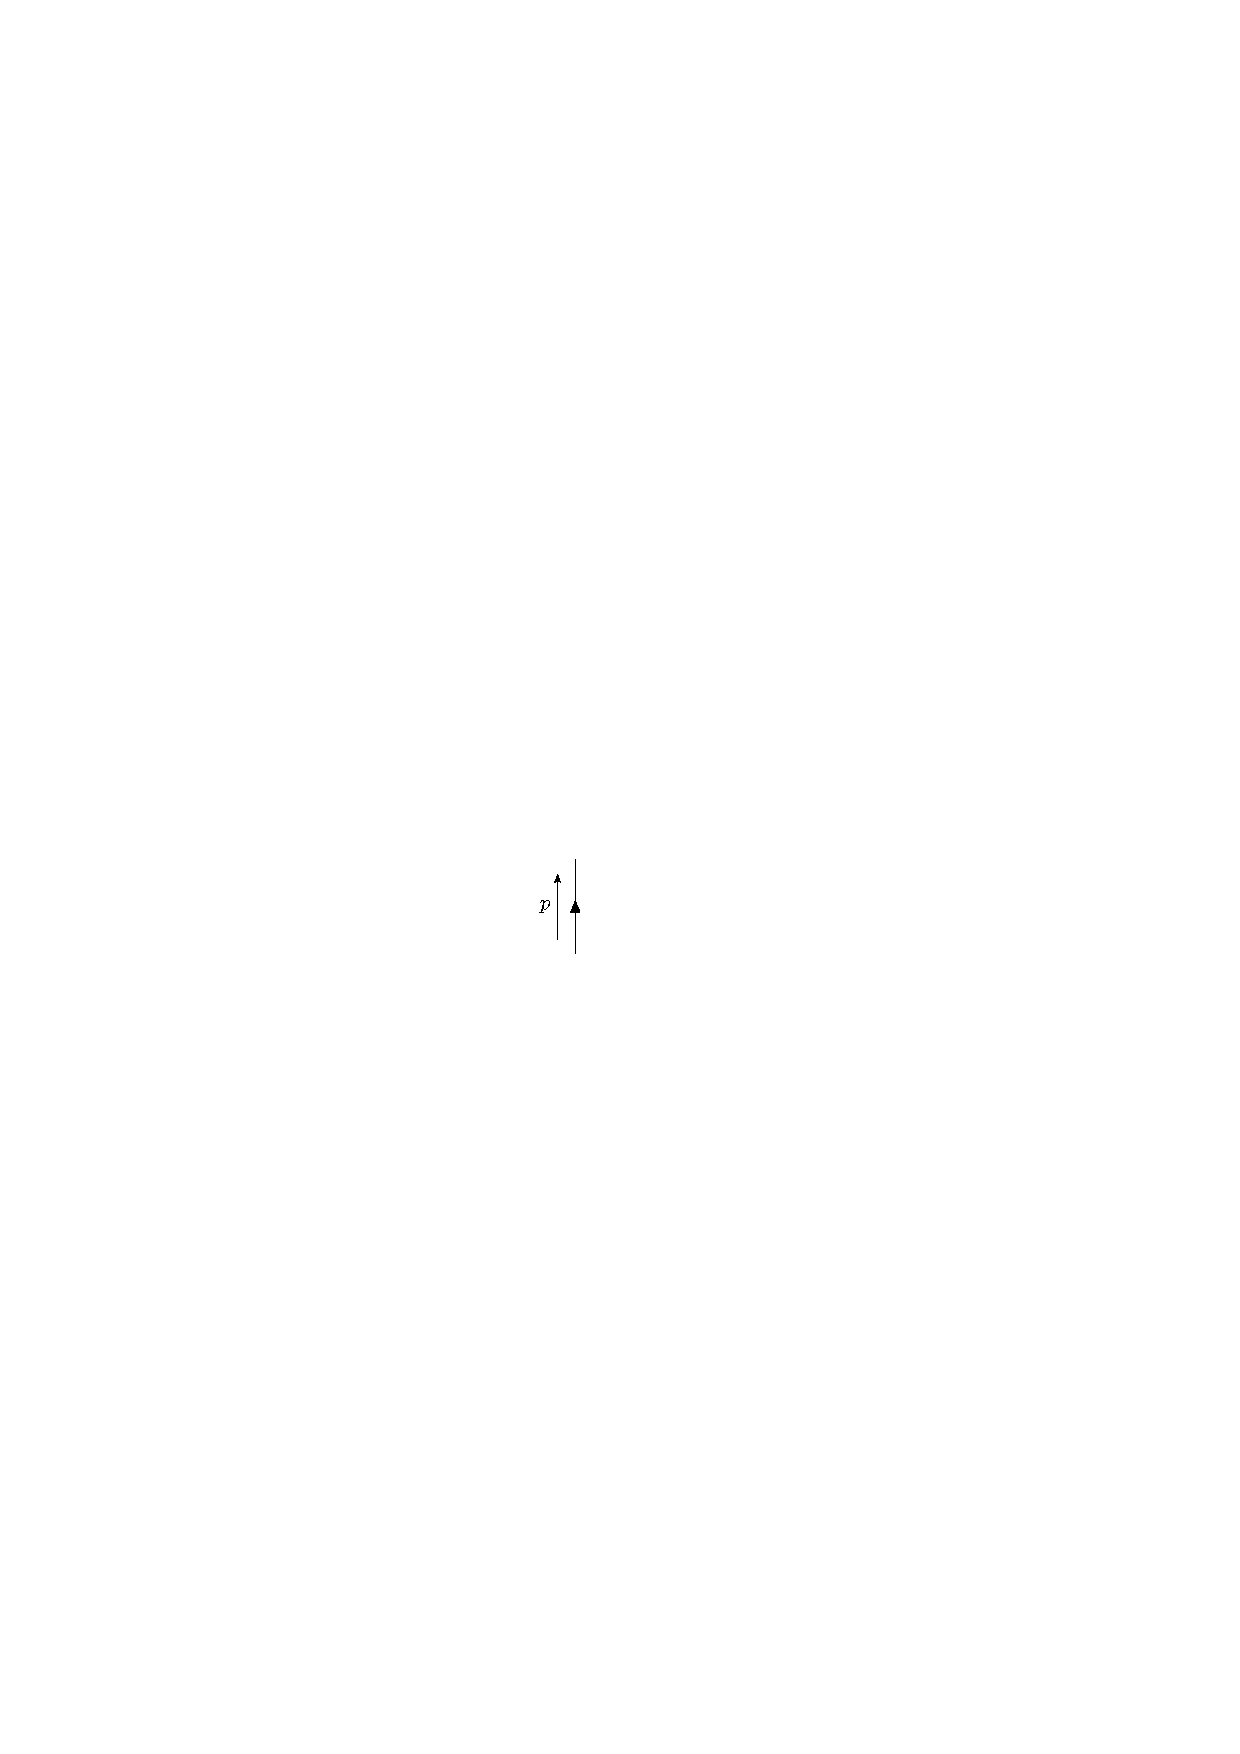
\includegraphics[scale=1]{figures/Yukawa interaction - Feynman diagram 1.pdf}}} =& (2 \pi)^4 \delta^{(4)}(p_1 + p_2) \Big( \frac{i}{\cancel{p}_1 - m + i \epsilon} \Big)_{\alpha \beta}, \\
		\vcenter{\hbox{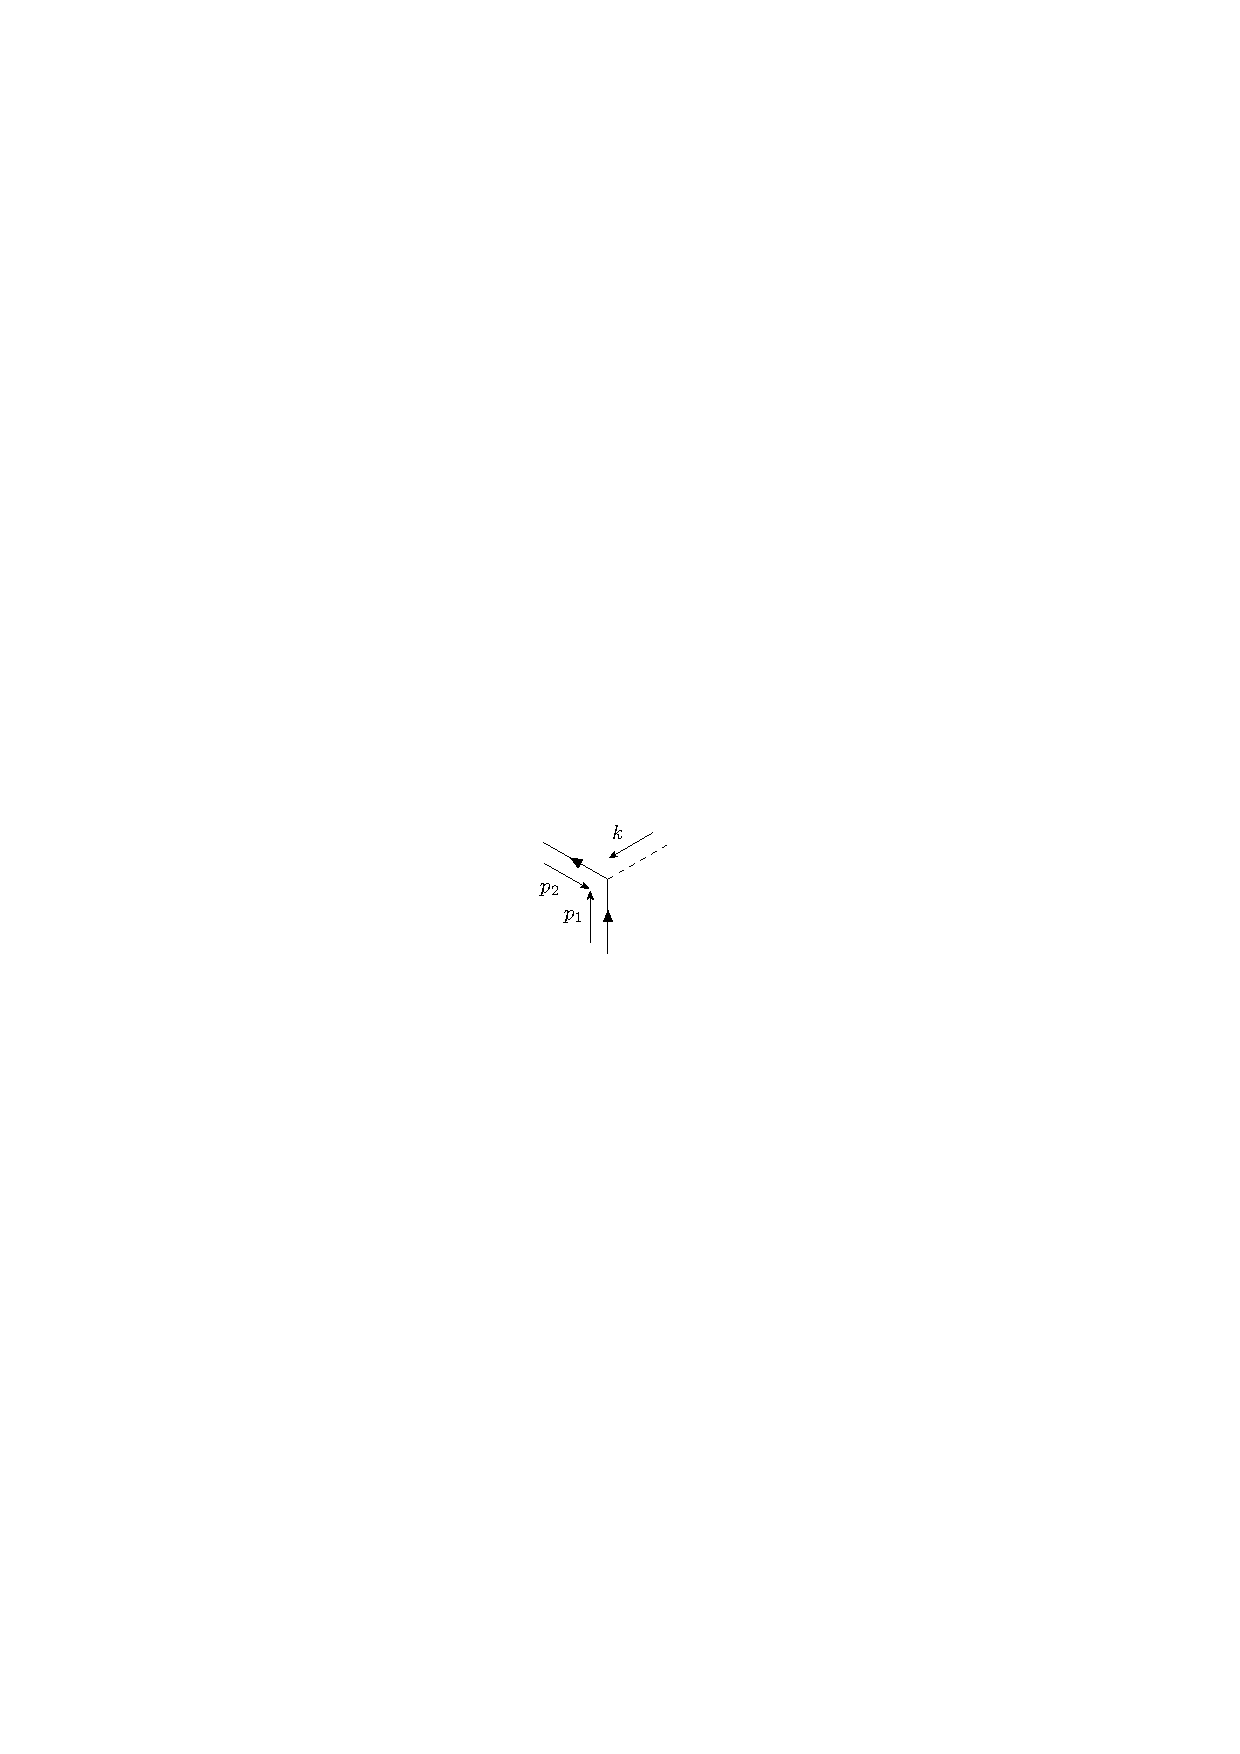
\includegraphics[scale=1]{figures/Yukawa interaction - Feynman diagram 2 (Weyl's way).pdf}}} =& i g (2 \pi)^4 \delta^{(4)}(p_1 + p_2 + k) \Big( \frac{i}{\cancel{p_1} - m + i \epsilon} \frac{i}{- \cancel{p_2} - m + i \epsilon} \Big)_{\alpha \beta} \frac{i}{k^2 - \mu^2 + i \epsilon},
	\end{align}
	
	\begin{tcolorbox}[title=calculation:]
		\begin{align}
			\vcenter{\hbox{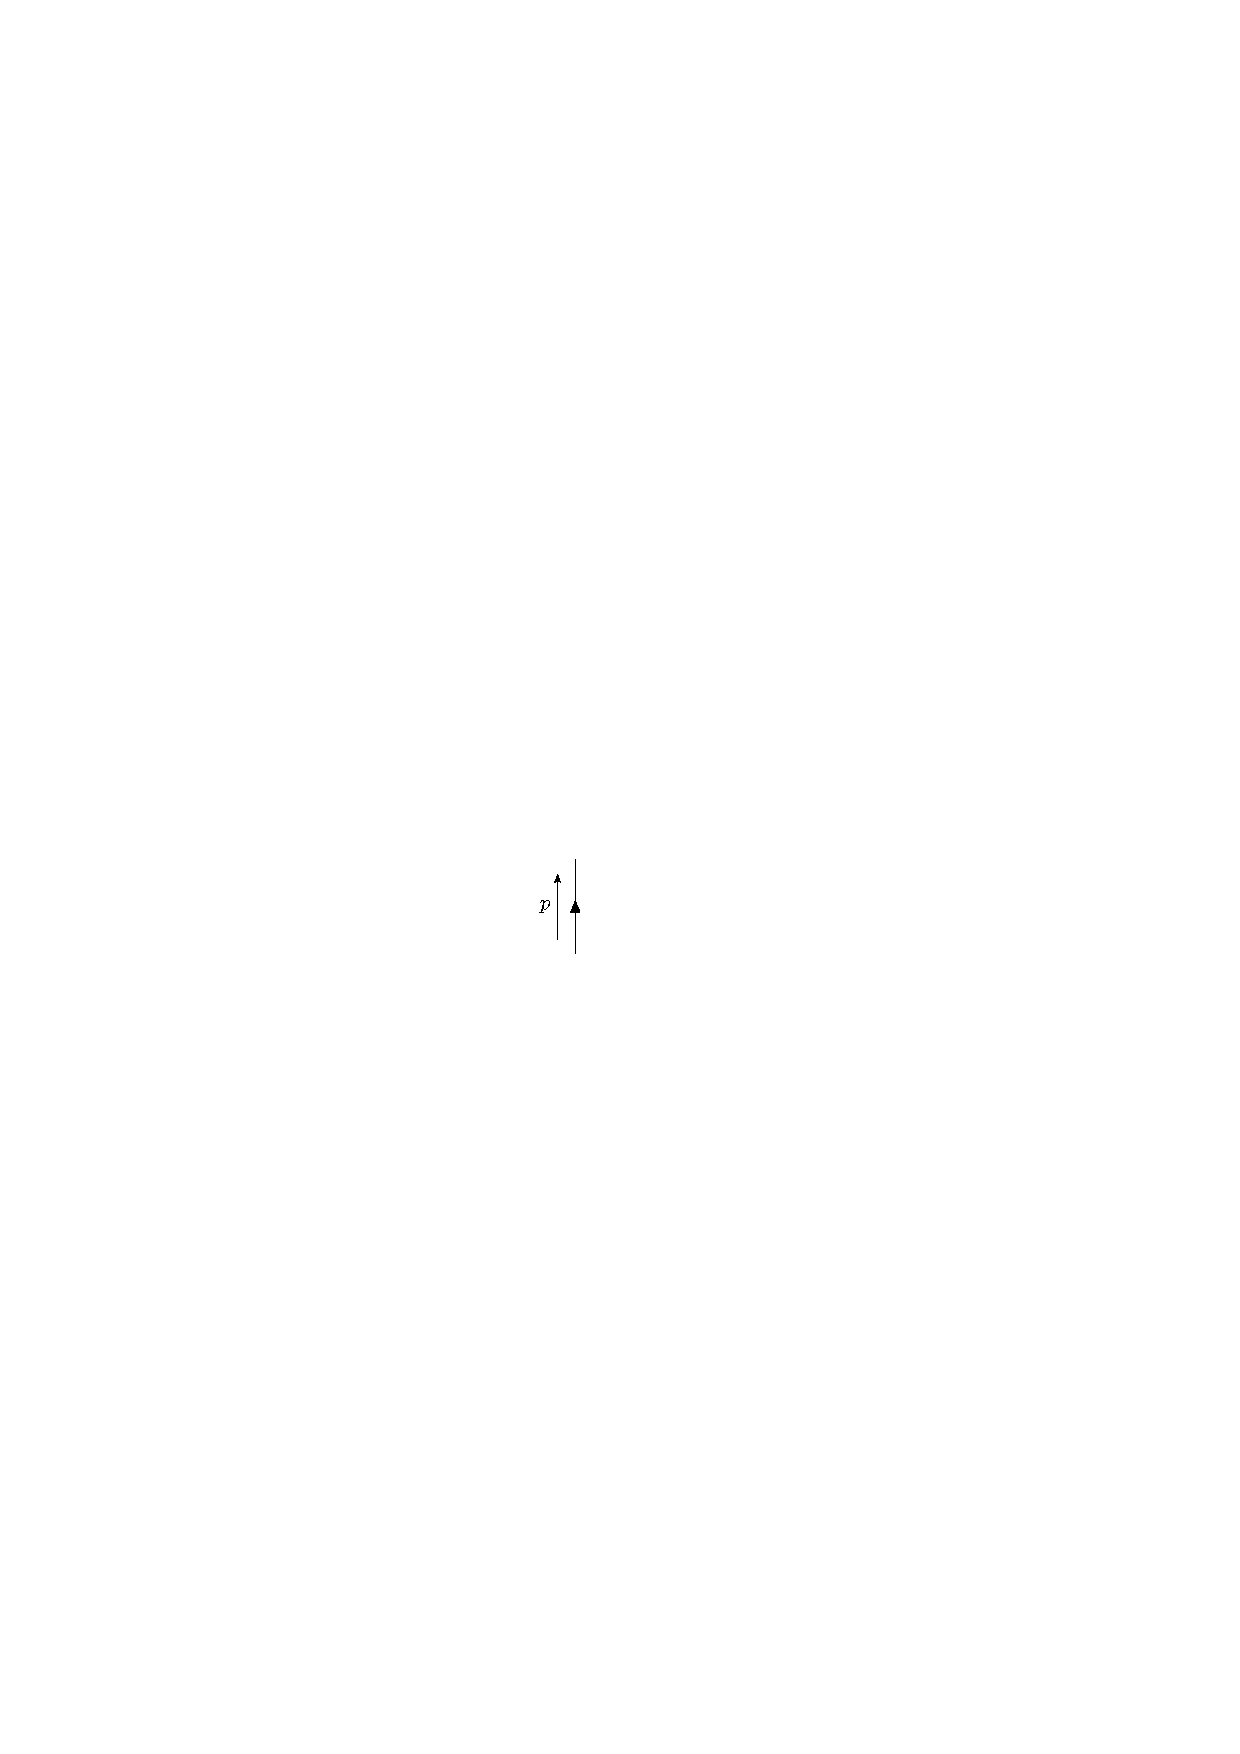
\includegraphics[scale=1]{figures/Yukawa interaction - Feynman diagram 1.pdf}}} =& \int d^4 x d^4 y \, e^{i p_1 \cdot x + i p_2 \cdot y} \braket{\wick{
				\c1 \Psi_\alpha(x) \c1 {\bar{\Psi}}_\beta(y)
			}} \notag \\
			=& \int d^4 x d^4 y \, e^{i p_1 \cdot x + i p_2 \cdot y} (- i)^2 (- i S_{\alpha \beta}(x - y)) = \cdots, \\
			\vcenter{\hbox{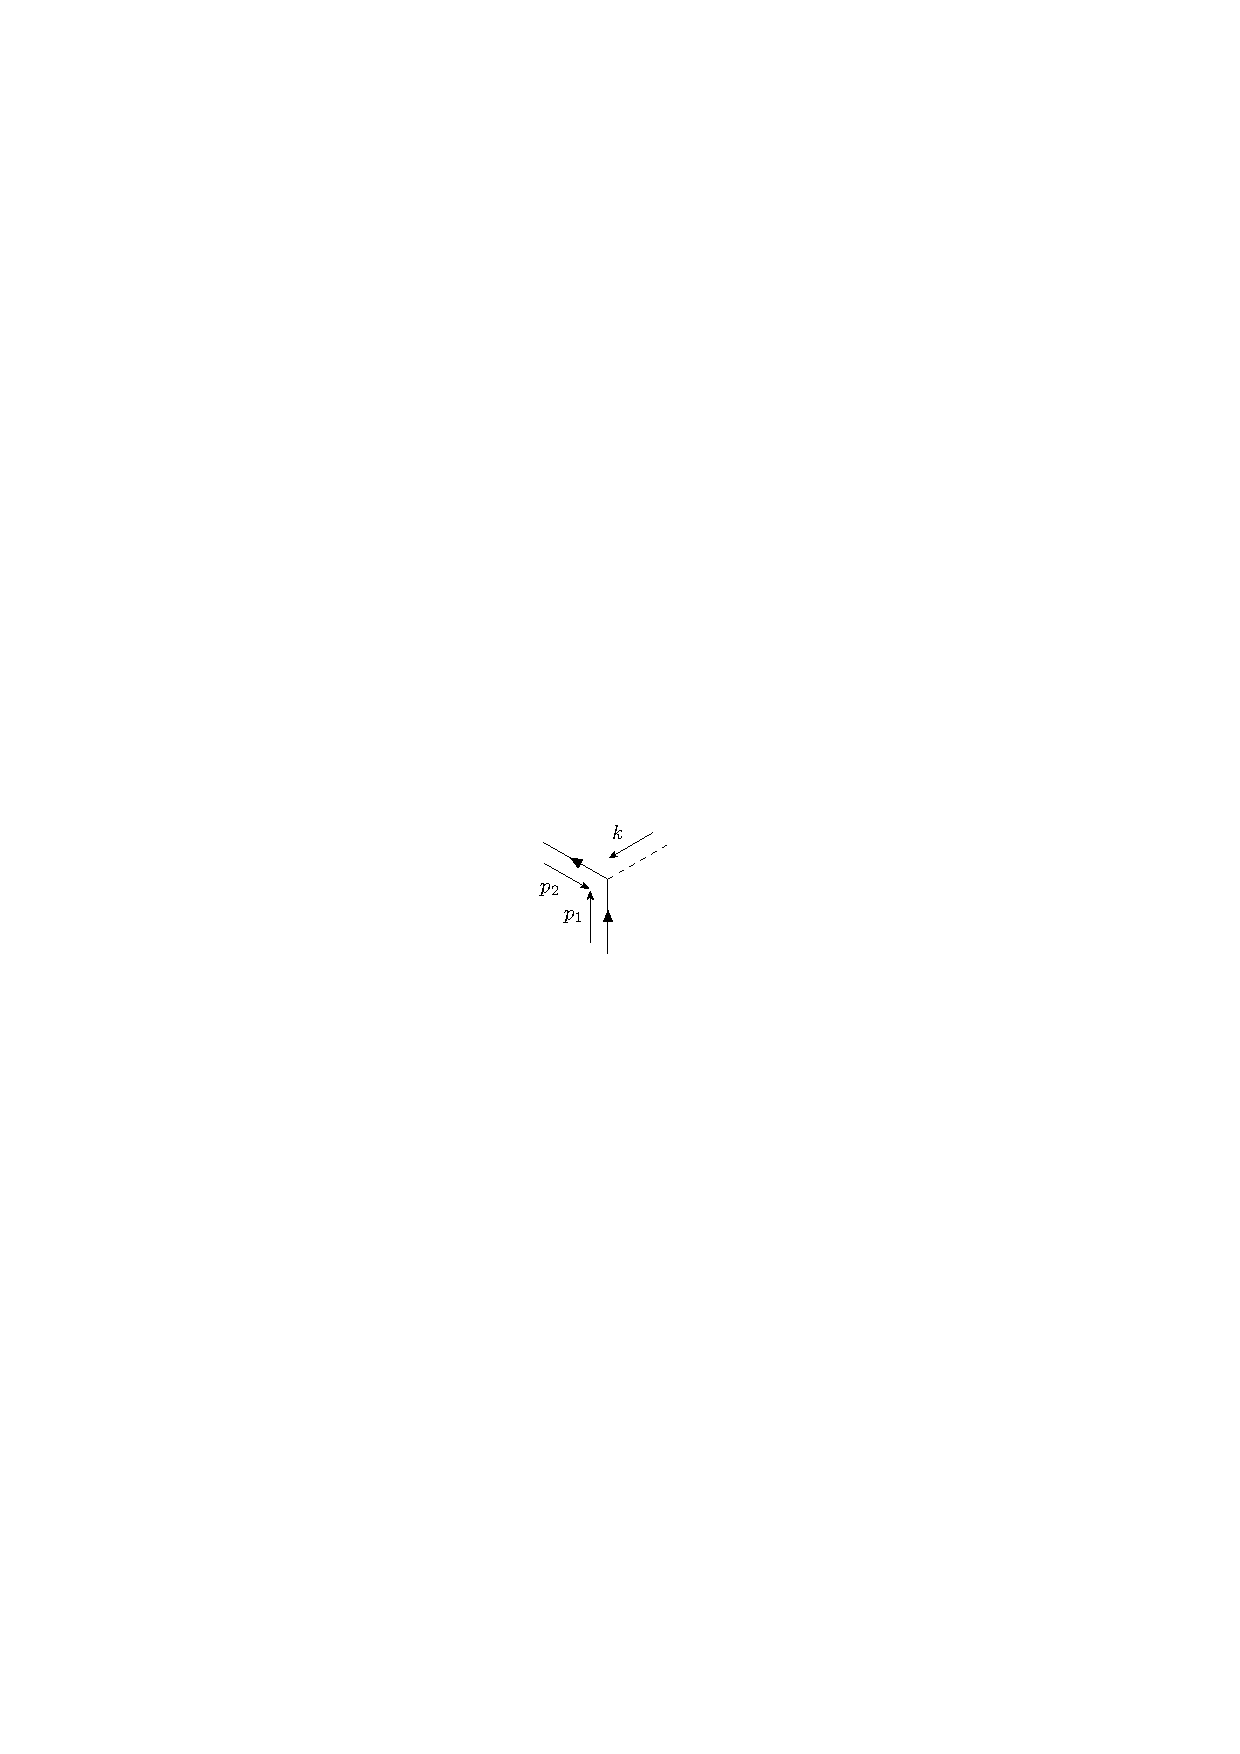
\includegraphics[scale=1]{figures/Yukawa interaction - Feynman diagram 2 (Weyl's way).pdf}}} =& \int d^4 x_1 d^4 x_2 d^4 y \, e^{i p_1 \cdot x_1 + i p_2 \cdot x_2 + i k \cdot y} \notag \\
			& \int d^4 z \, \braket{\wick{
				(i g \c1 {\bar{\Psi}}_\gamma(z) \c3 \phi(z) \c2 \Psi_\gamma(z)) \c3 \phi(y) \c1 \Psi_\alpha(x_1) \c2 {\bar{\Psi}}_\beta(x_2)
			}} \notag \\
			=& i g \int d^4 x_1 d^4 x_2 d^4 y \, e^{i p_1 \cdot x_1 + i p_2 \cdot x_2 + i k \cdot y} \notag \\
			& \int d^4 z (- (- i)^2 i S_{\alpha \gamma}(x_1 - z)) (- (- i)^2 i S_{\gamma \beta}(z - x_2)) (- (- i)^2 i D(z - y)) \notag \\
			=& i g \int d^4 z \, \Big( \frac{i e^{i p_1 \cdot z}}{\cancel{p}_1 - m + i \epsilon} \frac{i e^{i p_2 \cdot z}}{- \cancel{p}_2 - m + i \epsilon} \Big)_{\alpha \beta} \frac{i e^{i k \cdot z}}{k^2 - \mu^2 + i \epsilon} = \cdots
		\end{align}
	\end{tcolorbox}
	
	再算 \eqref{10.2.5},
	\begin{align}
		\vcenter{\hbox{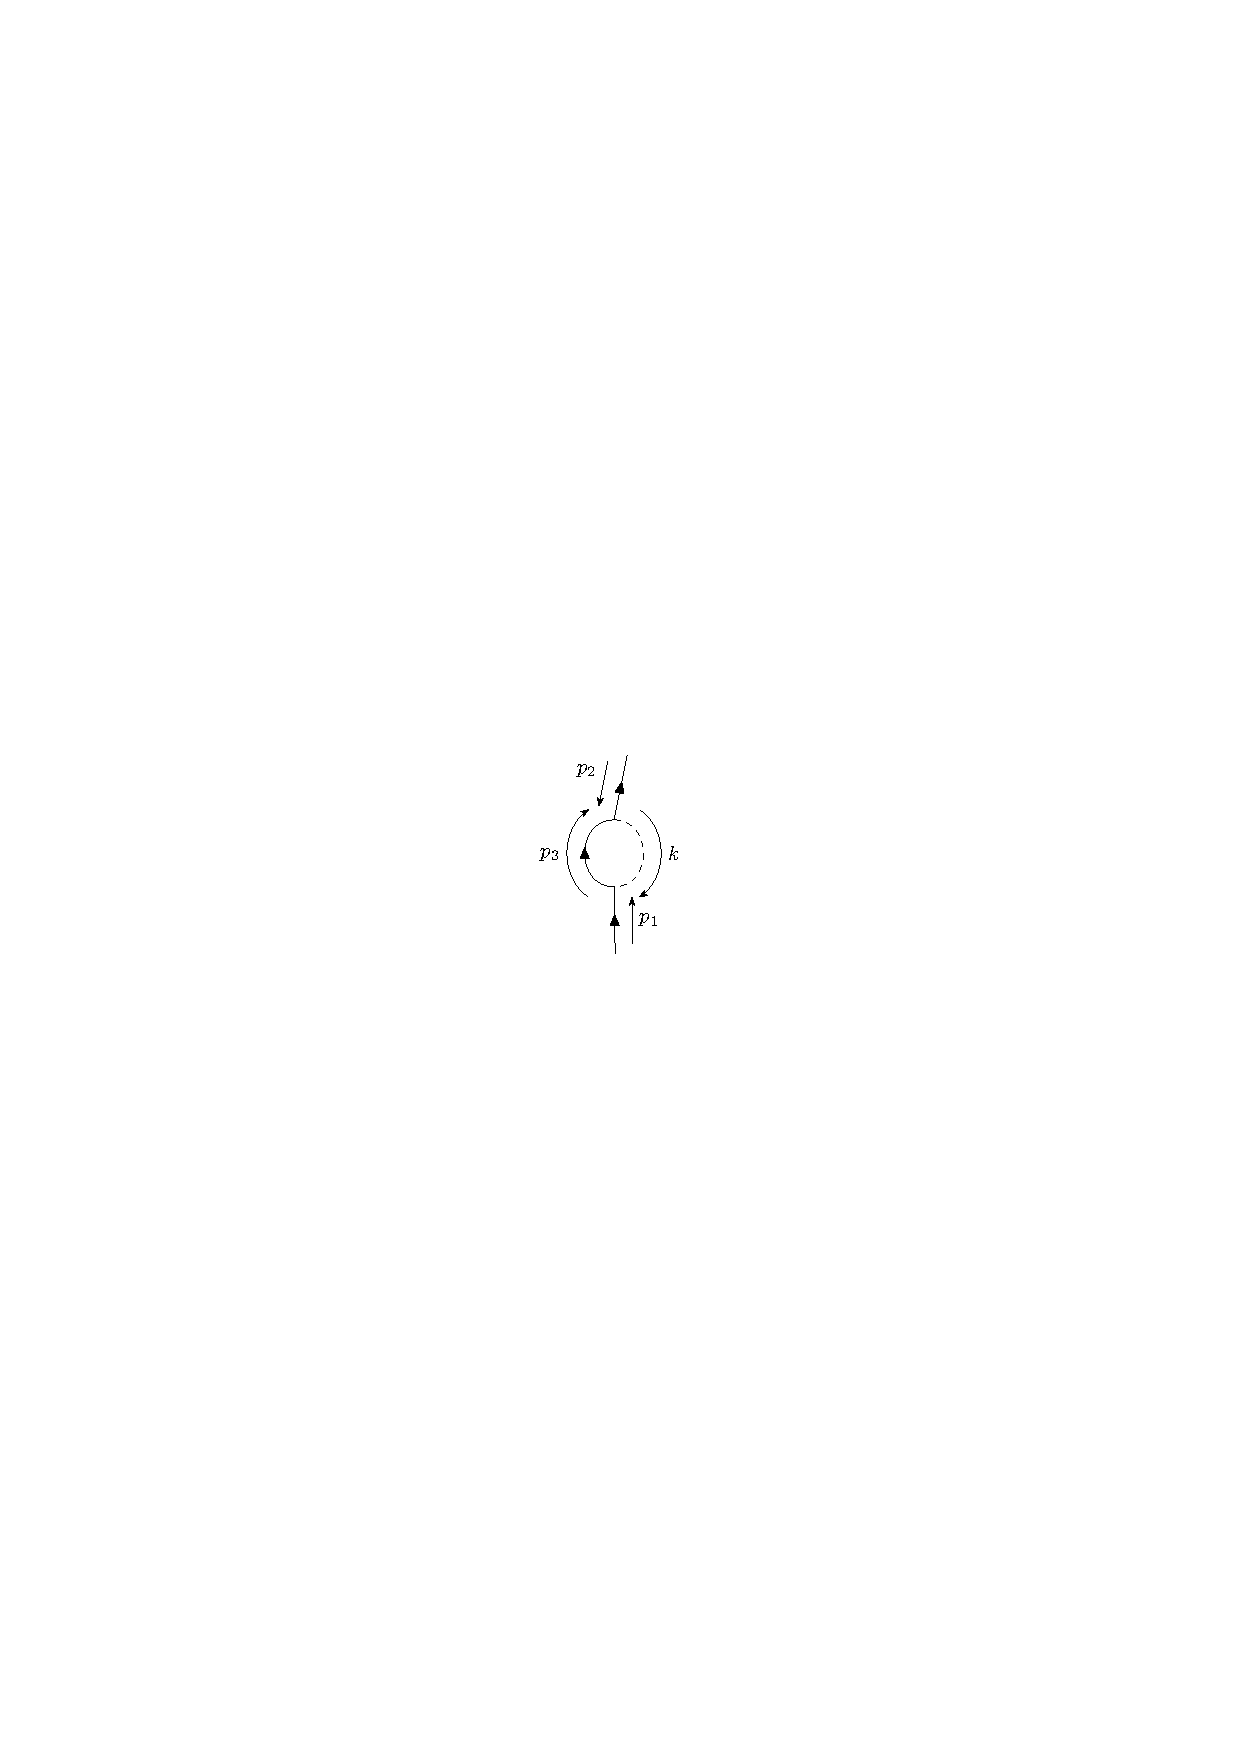
\includegraphics[scale=1]{figures/Yukawa interaction - Feynman diagram 3 (Weyl's way).pdf}}} =& (i g)^2 (2 \pi)^4 \delta^{(4)}(p_1 + p_2) \notag \\
		& \frac{i}{\cancel{p}_1 - m + i \epsilon} \int \frac{d^4 p_3}{(2 \pi)^4} \Big( \frac{i}{\cancel{p}_3 - m + i \epsilon} \frac{i}{(p_1 - p_3)^2 - \mu^2 + i \epsilon} \Big) \frac{i}{\cancel{p}_2 - m + i \epsilon}.
	\end{align}
	
	\begin{tcolorbox}[title=calculation:]
		\begin{align}
			& \cdots \notag \\
			=& \frac{(i g)^2}{2!} \int d^4 x_1 d^4 x_2 d^4 y_1 d^4 y_2 \, e^{i p_1 \cdot x_1 + i p_2 \cdot x_2} \Big( \braket{\wick{
				(\c1 {\bar{\Psi}}(y_1) \c4 \phi(y_1) \c3 \Psi(y_1) \c3 {\bar{\Psi}}(y_2) \c4 \phi(y_2) \c2 \Psi(y_2)) \c1 \Psi_1 \c2 {\bar{\Psi}}_2
			}} \notag \\
			& + (y_1 \leftrightarrow y_2) \Big) \notag \\
			=& (i g)^2 \int d^4 x_1 d^4 x_2 d^4 y_1 d^4 y_2 \, e^{i p_1 \cdot x_1 + i p_2 \cdot x_2} i S(x_1 - y_1) i S(y_1 - y_2) i S(y_2 - x_2) i D(y_1 - y_2) \notag \\
			=& (i g)^2 (2 \pi)^4 \delta^{(4)}(p_1 + p_2) \notag \\
			& \frac{i}{\cancel{p}_1 - m + i \epsilon} \int \frac{d^4 p_3}{(2 \pi)^4} \Big( \frac{i}{\cancel{p}_3 - m + i \epsilon} \frac{i}{(p_1 - p_3)^2 - \mu^2 + i \epsilon} \Big) \frac{i}{\cancel{p}_2 - m + i \epsilon}.
		\end{align}
	\end{tcolorbox}
\end{itemize}
